\begin{figure}[h]
\centering
    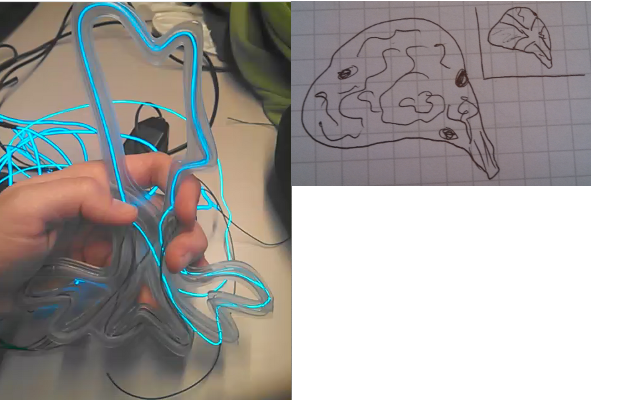
\includegraphics[width=3.4in]{figures/placeholder/teaser.png}
\caption{A novel neon sign (a) and a touch-sensitive brain (b) designed with our pipe tool and fabricated on a consumer-grade 3D printer.  (c) and (d) show the structure of the internal pipes generated by our tool.  \bjoern{will this be the robot or the UIST sign?} \valkyrie{arguably, the robot will be nicer-looking.  I think I'm manufacturing the UIST sign on the Makerbot.}}
\label{fig:teaser}
\end{figure}

\section{Introduction}
Makers, as well as professional designers, leverage 3D printers as tools for design work.  A wide array of objects, ranging from bicycle helmets to video game controllers, are now prototyped or even manufactured using these machines.  However, most devices fabricated by 3D printers are passive, prototyping the form, but not the interactivity, of an object.  

Due to the growing popularity of 3D printing and maker communities like Thingiverse\footnote{http://thingiverse.com}, recent work has looked at the issue of rapidly prototyping interactive objects. Existing approaches include Printed Optics \cite{Willis-printedoptics}, which uses optically clear material for light redirection, and Sauron \cite{Savage-sauron}, which is based on computer vision, but they are limited to visible interactions only; they do not give designers freedom to integrate haptic or acoustic inputs or outputs.

We propose a novel technique involving the removal of material from the interior of 3D models, prior to printing, to create pipes and other cavities.  These pipes can be filled, post-print, by a variety of media that enable input, display, and tactile feedback.  This {\em subtractive} approach is complementary to {\em additive} approaches that inject custom print materials, such as conductors, during the actual printing process [ref]. While our approach requires some manual assembly after a print completes, it gives makers the opprotunity to rapidly prototype a diverse range of interactive objects on 3D printers, including hobbyist machines (Figure \ref{fig:teaser}).

We describe a new design space of pipes and hollow chambers for the prupose of interaction design, where variables include openings, topologies, and inserted media. By exploring this design space new opportunities for adding interactivity to 3D printed objects can be realized. For example, copper material can fill the channels, to allow for standard electronic components to be easily integrated after the printout; electroluminescent (EL) wire can be threaded through to create computer-controlled visual output; or air can be pumped through to control haptic responses.  In comparison to traditional exterior electronics integration, our process allows makers to preserve aesthetics by hiding wires inside the object; additionally it offers more freedom in selecting precise surface locations for, e.g., air mediated tactile output.

\tovi{I would remove this entire paragraph} \valkyrie{I think we at least need to preserve the sentiment from the end, that we don't have any novel I/O techniques but that pipes help extend existing techniques in useful ways}
Pipes allow makers to build with and upon existing input/output techniques, often integrating these methods into objects they were not originally designed for.   For example, to create a touch-sensitive toy as in Figure \ref{fig:teaser}, a maker can select several locations of interest on the brain.  After creating pipes to those locations and printing her object, she can fill the pipes with conductive paint.  For sensing, she need only connect a single wire to a shared out of all the tubes, and can distinguish them via Swept Frequency Capacitve Sensing \cite{Sato-touche}.  In this way, she has only a single active element (the microcontroller setup), but her otherwise-inert 3D printed object (the brain) has several sensing locations.  Other existing sensing and actuation approaches, such as FlyEye \cite{Wimmer-flyeye} and Jamming User Interfaces \cite{Follmer-jamming}, can also be enhanced by the use of pipes: makers utilizing such I/O strategies can locate input and output at arbitrary points on an print's surface.  We leverage these existing techniques for sensing and actuation while our work's novelty is in \emph{internal modeling} for 3D printing and the \emph{redirection} of I/O to arbitrary locations on a device.

\tovi{I would remove this entire paragraph}  \valkyrie{if we scrap the first one, sure.  George, what do you think?}
Pipes can also be used for sending media on a specified route through an object; for example, neon signs are created by evacuated glass tubes formed into a specific path.  Electricity is run through the near-vacuum, creating light.  If our maker wants to build such a sign, she can substitute EL wire for the evacuated glass: she need only design a path for it to be fed through and then create pipes along that path.

Generating these pipes, however, is not trivial.  For one, most 3D modelling tools do not provide extensive tools for modelling the  {\em interior} of 3D models. Furthermore, careful consideration needs to go into the design and routing of the pipes. Pipes need maximum possible bend radius to ease the insertion of media post-print.  Independent pipes cannot intersect, as this could lead to electrical shorting or other problems.  Pipes should not pass too close to the surface: consumer-grade 3D printers do not guarantee air- or water-tightness of prints, so more than one printed layer may be required to prevent leakage.  Pipes for applications like neon signs must have a Euler tour through them: this allows a single EL wire to light every edge on the pipe graph.  No tools currently exist for these design tasks.  

Our work makes several contributions to the field of digitally fabricated interactive objects. First, we describe a design space of how pipes can be integrated into 3D models. We then offer algorithms and techniques for routing the pipes, and integrate these tools into  a 3D modelling applicaiton. The system takes into considertation the design complexities of routing interior pipes which are described above. Finally, we showcase a set of examples, enabled by our modeling tool, which allows us to explore various points in the design space. We conlcude by summarizing the input and out modalities enabled by our work, and discussing limitations and areas for future exploration. 
